\documentclass[11pt]{article}
\usepackage[margin=1in, top=0.5in]{geometry}
\usepackage[all]{nowidow}
\usepackage[hyperfigures=true, hidelinks, pdfhighlight=/N]{hyperref}
\usepackage[group-digits=false]{siunitx}
\usepackage{graphicx,amsmath,physics,tabto,float,amssymb,pgfplots,verbatim,tcolorbox}
\usepackage{listings,xcolor,subfig,keyval2e,caption,import,svg,wrapfig,lipsum}
\usepackage[version=4]{mhchem}
\numberwithin{equation}{section}
\numberwithin{figure}{section}
\numberwithin{table}{section}
\definecolor{stringcolor}{HTML}{C792EA}
\definecolor{codeblue}{HTML}{2162DB}
\definecolor{commentcolor}{HTML}{4A6E46}
\lstdefinestyle{appendix}{
    basicstyle=\ttfamily\footnotesize,commentstyle=\color{commentcolor},keywordstyle=\color{codeblue},
    stringstyle=\color{stringcolor},showstringspaces=false,numbers=left,upquote=true,captionpos=t,
    abovecaptionskip=12pt,belowcaptionskip=12pt,language=Python,breaklines=true,frame=single}
\lstdefinestyle{inline}{
    basicstyle=\ttfamily\footnotesize,commentstyle=\color{commentcolor},keywordstyle=\color{codeblue},
    stringstyle=\color{stringcolor},showstringspaces=false,numbers=left,upquote=true,frame=tb,
    captionpos=b,language=Python}
\renewcommand{\lstlistingname}{Appendix}
\pgfplotsset{compat=1.17}

\begin{document}
    \begin{center}
        {\huge Identifying nuclides by their gamma ray spectra}\\
        \vspace{0.2in}
        \textbf{KDSMIL001 | May 2021}
        
        \section*{Abstract}\label{sec:Abstract}
        We analyse the gamma ray spectra of known nuclides and compare our results to the expected values in order to calibrate our set-up for identifying unknown samples by their gamma ray spectra. We determine that an unknown nuclide's gamma ray spectrum has a singular photopeak corresponding to an energy of $\SI{842(31)}{k\electronvolt}$. This is most likely \ce{^{54}Mn}.
    \end{center}

    \section{Introduction}\label{sec:Introduction}
    \par In this lab, we investigate the process known as Gamma Ray Spectroscopy, whereby we are able to identify various radioactive nuclei by the signature gamma rays that are emitted when they decay by the $\beta+$ or $\beta-$ decay mode. We are interested in gamma rays with energy between about 50 and 2000 keV.

    \section{Theory}\label{sec:Theory}
    \par When a nuclide decays, it can decay in one of a few ways. The decay modes we are interested in are called $\beta$ decays, where the nucleus either gains a proton and loses a neutron, or loses a proton and gains a neutron, changing elemental structure. When this happens, in order to conserve the charge of a proton being created or destroyed, we see a $\beta$ particle (positive or negative depending on the decay mode) emitted along with a neutrino or antineutrino. After the decay, if we sum up the masses of the resulting nuclide, $\beta$ particle, and neutrino, we see that the total is less than the mass of the nuclide before the decay. This missing energy is usually accounted for by the resulting nuclide being in an excited state and when it transitions to a lower energy state, it emits a photon. These are the photons we are detecting.
    \par Our detector is a scintillator detector, meaning it absorbs the incident gamma rays and emits rays of proportional but lesser energy, to be absorbed by a photomultiplier tube, whose signal is amplified by an array of amplification devices. In a perfect world this system would produce current pulses that are proportional only to the incident gamma rays, but since we don't live in a perfect world we see pulses corresponding to secondary processes that end up on our spectra. The main processes of concern are photoelectric absorption, Compton scattering, pair production, and backscatter, on which more details can be found in (Gilmore Ch 2.2) \cite{gilmore}. 
    \par The detector and amplifier set-up leads into either an oscilloscope or a Multi Channel Analyser (MCA), allowing us to observe the current pulses. The MCA counts the number of times that a pulse of a certain voltage is detected and plots that on a histogram, giving us our  spectrum for the given radioactive source. These spectra, to a certain degree, are unique to the nuclide that decayed to produce them, and thus we should be able to identify an unknown radioactive source purely from its gamma ray spectrum.

    \section{Method}\label{sec:Method}
    \par We used the apparatus configured as in \autoref{fig:Apparatus}. The detector is an NaI scintillator detector and photomultiplier tube. The preamplifier is an ORTEC model 113. The amplifier is an ORTEC model 572. The MCA is a SPECTECH UCS-30 running with 1024 channels. 
    \begin{wrapfigure}{r}{.5\textwidth}
        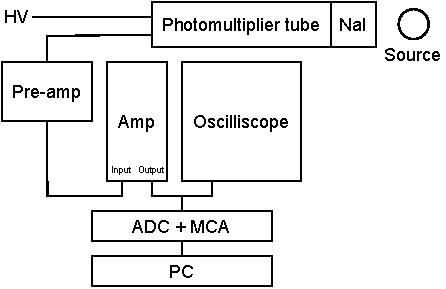
\includegraphics{apparatus.pdf}
        \caption{Schematic of the set-up used in the experiment.}
        \label{fig:Apparatus}
    \end{wrapfigure}
    \par The oscilloscope was used to monitor the voltage of the current pulses produced by the amplifier. The MCA has a maximum input voltage of 5V, so the gain on the amplifier was changed in order to keep all pulses of interest below 5V. 
    \par The radioactive sources we analysed were the following: \ce{^{22}Na}, \ce{^{60}Co}, \ce{^{109}Cd}, \ce{^{133}Ba}, \ce{^{137}Cs}, \ce{^{152}Eu}, and an unknown source. We started by letting the MCA run for a while to collect background data. Then we placed each source in front of the detector and let the MCA collect data for between 10 minutes to an hour on each source. 

    \section{Analysis}\label{sec:Analysis}
    \par The data exported by the MCA tells us how many times a current pulse reached the detector within the time spent collecting data, discretised into channels. We normalised these counts with respect to the time spent collecting data, namely the live time as it accounts for the shaping time of the MCA, and then subtracted the background data from them to try to get a cleaner signal. Plotting this data as a histogram we were then able to identify the photopeaks by eye and find an approximate range of channels on which the plot resembles a gaussian distribution. We could then use \texttt{scipy.optimize.curve\_fit} to fit a gaussian function to the data on those regions in order to approximate a mean for each photopeak. \autoref{fig:Cs and Na spectra} shows two of our samples' spectra. 

    \begin{figure}[H]%
        \centering
        \subfloat[\centering \ce{^{137}Cs} gamma ray spectrum using an NaI scintillator detector.]{\scalebox{0.4}{\subimport{Plots}{137Cs.pgf}}}
        \,
        \subfloat[\centering \ce{^{22}Na} gamma ray spectrum using an NaI scintillator detector.]{\scalebox{0.4}{\subimport{Plots}{22Na.pgf}}}
        \caption{Gamma ray spectra for 2 of the radioactive sources to demonstrate the process of finding $\mu$ and $\sigma$.}
        \label{fig:Cs and Na spectra}
    \end{figure}

    \par As our goal was to identify the unknown source, we wanted to be able to accurately estimate the energy associated with its photopeak. In order to do this we needed to find a relation between MCA channel number and photon energy. We found the approximate voltage of the centroid value of each clearly identifiable peak (voltage is associated with channel number by a scaling factor of 5/1024) and then found the expected energy of that peak using the Nudat2 database \cite{nudat} and could then correlate the two with a linear least squares regression, as in \autoref{fig:linear regression}.

    \begin{figure}[H]%
        \centering
        \subfloat{\scalebox{0.5}{\subimport{Plots}{linearRegression.pgf}}}
        \,
        \resizebox{6.5cm}{!}{
        \begin{tabular}[b]{| c | c | c |}\hline
            & Channel & Expected Energy [keV]\\\hline
            \ce{^{22}Na} & \num{320(15)} & \num{511}\\
             & \num{782(24)} & \num{1274.537(7)}\\\hline
            \ce{^{60}Co} & \num{735(26)} & \num{1173.228(3)}\\
             & \num{835(23)} & \num{1332.494(4)}\\\hline
            \ce{^{109}Cd} & \num{55.2(59)} & \num{88.0336(10)}\\\hline
            \ce{^{133}Ba} & \num{49.1(82)} & \num{88.9979(11)}\\
             & \num{228(16)} & \num{356.0129(7)}\\\hline
            \ce{^{137}Cs} & \num{417(16)} & \num{661.657(3)}\\\hline
            \ce{^{152}Eu} & \num{76(10)} & \num{121.7817(3)}\\
             & \num{155(20)} & \num{244.6974(8)}\\
             & \num{219(16)} & \num{344.2785(12)}\\\hline
            Unknown & \num{527(17)} & \num{843(31)}\\\hline
        \end{tabular}
        }
        \caption{Correlating detected voltage with gamma ray energy. Note the expected energies are from Nudat2 \cite{nudat} except for the energy of the unknown source, which is calculated below.}
        \label{fig:linear regression}
    \end{figure}

    \par We then had our calibration equation:
    \begin{align}
        E_{\gamma}&=\frac{V-0.002}{0.003049}\label{eqn:calibration}\\
        u(E_{\gamma})&=E_{\gamma}\sqrt{\left(\frac{\sqrt{u(V)^2+0.022^2}}{V-0.002}\right)^2 + \left(\frac{0.000056}{0.003049}\right)^2}\label{eqn:calibration uncertainty}
    \end{align}
    where $E_\gamma$ has units $\si[]{k\electronvolt}$ and $V$ is the detected voltage. Using this equation we were able to determine an energy for the photopeak in \autoref{fig:unknown}: $E_\gamma=\SI{843(31)}{k\electronvolt}$. 

    \begin{wrapfigure}{R}{0.5\textwidth}
        \scalebox{0.5}{\subimport{Plots}{Unknown.pgf}}
        \caption{The unknown sample's gamma ray spectrum. Note that there appears to only be one photopeak of significant intensity, which narrowed down our search parameters.}
        \label{fig:unknown}
    \end{wrapfigure}

    \par When it comes to identifying which nuclide it is that produced this spectrum, it's not a particularly simple job. We begun by looking at the gamma ray table on \texttt{http://atom.kaeri.re.kr/} \cite{kaeri}, setting the bounds on energy to be the upper and lower bounds of our $68\%$ confidence interval and setting the minimum half life to 10 days. This gave us 19 results. Looking at all the results with a non-negligible intensity, 14 in total, we noticed that only one of the options had a single emitted gamma ray from ground state, and no $\SI{511}{k\electronvolt}$ annihilation gamma rays of significant intensity. This option was \ce{^{54}Mn}, whose only gamma ray emission of significant intensity is  of energy $\SI{834.848(3)}{k\electronvolt}$ with intensity $99.9760(10)\%$ \cite{nudat}. 
    \clearpage
    
    \section{Conclusion}\label{sec:Conclusion}
    \par We were able to find a calibration equation for our experimental set-up, \autoref{eqn:calibration} and \autoref{eqn:calibration uncertainty}, which allowed us to determine the energy of a photopeak in the gamma ray spectrum of an unknown source. The peak was at channel number \num{527(17)}, which corresponds to an energy of $\SI{843(31)}{k\electronvolt}$. Using \texttt{http://atom.kaeri.re.kr/} \cite{kaeri} we were able to find a most likely nuclide, \ce{^{54}Mn}.

    \begin{thebibliography}{9}
        \bibitem{gilmore}
        Gordon Gilmore. (2008). \textit{Practical Gamma-ray Spectrometry}. 2. Chichester: Wiley
        \bibitem{nudat}
        Nudat 2. Nndc.bnl.gov. \texttt{https://www.nndc.bnl.gov/nudat2/chartNuc.jsp}
        \bibitem{kaeri}
        Nuclear Data Center at KAERI. Atom.kaeri.re.kr. \texttt{http://atom.kaeri.re.kr/}
    \end{thebibliography}
    

\end{document}